\chapter{Eigen Value Analysis}

Eigenvalues tells about how the given system matrix $\vec{A}$ will respond or evolve in the particular direction of Eigenvectors. Consider a system matrix given by
\begin{equation}
	\vec{A} = \begin{bmatrix}
	1 & 0 \\ 0 & -1
	\end{bmatrix}
\end{equation}
the Eigenvalues and the Eigenvectors of the system are given by
\begin{align*}
	\lambda_{1} & = 1 \\
	\lambda_{2} &= -1 \\
	v_1 & =	\begin{bmatrix}
	1 \\ 0
	\end{bmatrix} \\
	v_2 & =	\begin{bmatrix}
	0 \\ 1
	\end{bmatrix}
\end{align*}
If the Eigenvectors are plotted on a simple scale along the horizontal and the vertical axis as shown in the figure \ref{Fig_EVA_EigenVectorPlot}
\begin{figure}[h!]
	\centering
	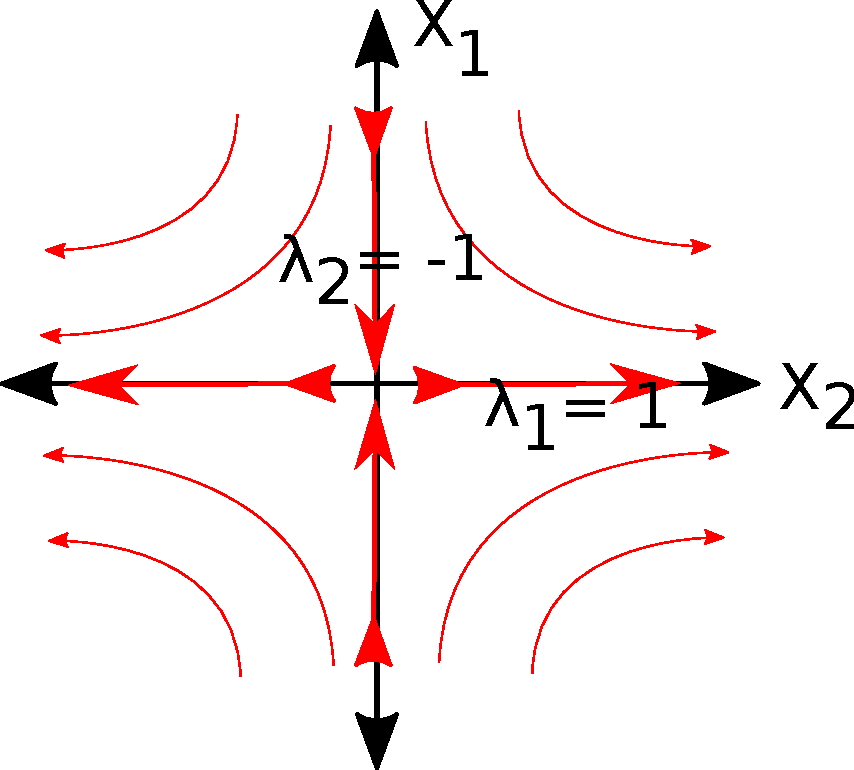
\includegraphics[width=\linewidth]{Bilder/EigenVectorPlot.pdf}
	\caption{Plot of Eigenvectors and the matrix A evolution along Eigenvectors}
	\label{Fig_EVA_EigenVectorPlot}
\end{figure}
\newpage
\textbf{Note: }The axis $x_1$ and $x_2$ in figure \ref{Fig_EVA_EigenVectorPlot} are interchanged !!!

suppose the system starts on the axis $x_2$ where $\lambda_{2} = -1$, the system dynamics will evolve towards the origin therefore, attenuating the dynamics and the system will be stable. However, if the system starts on axis $x_{1}$ where $\lambda_{1} = 1$, then the states will evolve towards positive side of the Eigenvector which will amplify the dynamics and therefore, the system will be unstable. At any other points, due $\lambda_{2} = -1$, the dynamics will move downwards and due to $\lambda_{1} = 1$, the states will evolve towards amplification, therefore the system as a whole will not be stable. One particular case, when the system starts exactly along the Eigenvector where $\lambda = -1$ is in the case of an inverted pendulum which is perfectly aligned vertically towards the line of gravity and will remain in that position unless an external disturbance is applied.

\section{How Eigen Value Analysis Works}

Using the definition of Eigen value,
\begin{equation}
	\vec{A}\vec{v} = \lambda \vec{v}
\end{equation}
which says that $\vec{A}$ is a matrix which acts as a scaling factor to the vectors $\vec{v}$, such that the scaling factor is $\lambda$. Now the scaling factor $\lambda$ is acing on $\vec{v}$ in order to scale this vector. How much this vector gets scaled and in which direction depends on the factor $\lambda$. Here $\vec{v}$ is called the Eigen vector and $\lambda$ is called the Eigen value. 

Therefore, there is now a relationship where it can be found the evolution of vector of $\vec{v}$ depending on the factor $\lambda$.
